% ============================================================================
% Week 5 -- LECTURE NOTE (student-facing)
%
% Merge of the old full-prose week03.tex (assignment, transportation, total
% unimodularity) and week04.tex (MCNF, facility location, the deterministic
% LAP), condensed to board fragments. Knapsack is NOT repeated here -- it was
% covered in week 2 (week02-03-note.tex, beat 3). Style of week02-03-note.tex.
% Self-contained -- no \input{preamble}.
% ============================================================================
\documentclass[10pt]{article}

\usepackage[a4paper, margin=1.5cm]{geometry}
\usepackage{amsmath, amssymb}
\usepackage[dvipsnames]{xcolor}
\usepackage{graphicx}
\usepackage{array}
\usepackage{tikz}
\usepackage{kotex}
\usepackage[hidelinks]{hyperref}

\definecolor{ruleink}{RGB}{18, 68, 140}
\definecolor{demoink}{RGB}{140, 82, 20}
\definecolor{keyink}{RGB}{20, 90, 20}
\definecolor{watchink}{RGB}{86, 60, 140}
\definecolor{punchink}{RGB}{170, 30, 60}

\setlength{\parindent}{0pt}
\pagestyle{empty}

% tighter spacing around centered displays
\AtBeginDocument{%
  \abovedisplayskip=4pt plus 1pt
  \belowdisplayskip=4pt plus 1pt
  \abovedisplayshortskip=2pt
  \belowdisplayshortskip=2pt}

% ---- one section -----------------------------------------------------------
\newcommand{\beat}[2]{%   number, title
  \par\medskip
  {\color{ruleink}\rule{\textwidth}{1pt}}\par\nobreak\vspace{2pt}
  {\large\bfseries #1.\; #2}\par\nobreak\vspace{3pt}}

% ---- board content ---------------------------------------------------------
\newenvironment{board}{%
  \par\vspace{2pt}
  \begingroup\leftskip=1.3em\relax}{%
  \par\endgroup\vspace{2pt}}

% ---- highlights ------------------------------------------------------------
\newcommand{\demo}[2]{\par{\color{demoink}\small\textbf{demo}\quad\texttt{#1} --- #2}\par}
\newcommand{\watch}[1]{\par{\color{watchink}\small\textbf{watch}\quad #1}\par}
\newcommand{\key}[1]{\par\vspace{1pt}{\color{keyink}\small\textbf{KEY}\quad\textbf{#1}}\par}
\newcommand{\takeaway}[1]{%
  \par\vspace{2pt}\noindent
  {\color{punchink}\rule{2pt}{10pt}}\;{\color{punchink}\small\textbf{takeaway}\quad\textbf{#1}}\par\vspace{2pt}}

\begin{document}

{\Large\bfseries Week 5 --- Classic IP Models, Networks, and the LAP}\\[2pt]
{\small OL7014 Integer Programming \quad\textbullet\quad Instructor: Prof.\ H.\ Park \quad\textbullet\quad Week of Sep 21, 2026}

% ---------------------------------------------------------------- 1
\beat{1}{Matching --- a model born canonical}
\demo{ip-games / assignment}{play FIRST: three pilots, three aircraft, one each. \ \url{https://hankpark0706.github.io/ip-games/assignment-matching.html}}
\begin{board}
3 pilots, 3 aircraft, one each --- or officers to billets, units to sectors, interpreters to teams.
$c_{ij}$ = value of the pairing $(i,j)$. \ this is the \textbf{assignment problem} {\footnotesize(할당 문제)} --- a perfect
\emph{matching} in a bipartite graph --- and the decision is a \emph{table}:
\[
  X \in \{0,1\}^{3\times 3}, \qquad x_{ij} = 1 \ \text{iff pilot } i \text{ flies aircraft } j
\]
rows sum to 1 (each pilot once), columns sum to 1 (each aircraft once):
\[
\begin{aligned}
  \max_X\quad & \langle C, X \rangle \\
  \text{s.t.}\quad & X \mathbf{1} = \mathbf{1}, \quad X^{\top}\mathbf{1} = \mathbf{1}, \quad X \ge 0
\end{aligned}
\]
\emph{read the symbols:} \ $\langle C, X \rangle = \sum_{i,j} c_{ij} x_{ij}$, \quad $\mathbf{1}$ = all-ones vector
\vspace{3pt}

matrix form by \textbf{flattening}: $x = \operatorname{vec}(X) \in \mathbb{R}^9$, \ $c = \operatorname{vec}(C)$
\ $\Rightarrow$ \ a $6 \times 9$ matrix of 0/1, \ $b = \mathbf{1}$
\vspace{3pt}

\quad \textbullet\ each column of $A$: exactly \textbf{two ones} --- one pilot row, one aircraft row \ (an \emph{incidence matrix})
\vspace{1pt}

\quad \textbullet\ binaries already gone: row sums $= 1$ with $x \ge 0$ cap every variable at 1
\vspace{1pt}

\quad \textbullet\ $\operatorname{rank} A = 5$: any one row is implied by the rest
\vspace{4pt}

\textbf{now run week 2's experiment again:} delete integrality, solve the LP, look at the answer
\vspace{2pt}

\quad it comes back a matching --- the LP always has an \emph{integral} optimum, and a vertex solver always returns one.
no cost table breaks it
\end{board}
\begin{center}
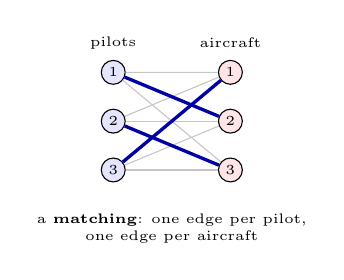
\begin{tikzpicture}[scale=0.62, font=\tiny, >=stealth]
  \foreach \i/\y in {1/2.0, 2/1.0, 3/0.0} {
    \node[circle, draw, fill=blue!10, inner sep=1.4pt] (p\i) at (0,\y) {$\i$};
    \node[circle, draw, fill=red!10, inner sep=1.4pt] (a\i) at (2.4,\y) {$\i$};}
  \node[font=\tiny] at (0,2.6) {pilots}; \node[font=\tiny] at (2.4,2.6) {aircraft};
  \foreach \i in {1,2,3} { \foreach \j in {1,2,3} { \draw[gray!45] (p\i) -- (a\j); } }
  \draw[very thick, blue!65!black] (p1) -- (a2);
  \draw[very thick, blue!65!black] (p2) -- (a3);
  \draw[very thick, blue!65!black] (p3) -- (a1);
  \node[align=center] at (1.2,-1.2) {a \textbf{matching}: one edge per pilot,\\ one edge per aircraft};
\end{tikzpicture}
\hspace{12mm}
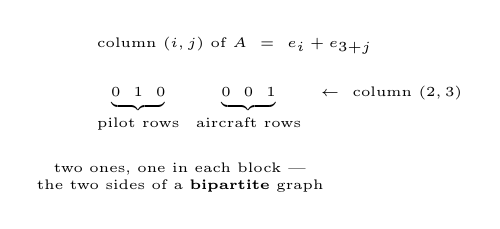
\begin{tikzpicture}[scale=0.62, font=\tiny]
  \node[anchor=west, align=left] at (0,1.5) {column $(i,j)$ of $A$ \ $=$ \ $e_i + e_{3+j}$};
  \node[anchor=west] at (0,0.2)
    {$\underbrace{0 \ \ 1 \ \ 0}_{\text{pilot rows}} \ \ \underbrace{0 \ \ 0 \ \ 1}_{\text{aircraft rows}}$
     \ \ $\leftarrow$ \ column $(2,3)$};
  \node[align=center] at (1.9,-1.2) {two ones, one in each block ---\\ the two sides of a \textbf{bipartite} graph};
\end{tikzpicture}
\end{center}
\key{$2n$ rows, $n^2$ variables, a harder-looking model than week 1's two-row toy --- and an \emph{easier} answer. something structural is going on.}
\takeaway{matching's LP returns whole numbers with no integrality declared. the reason has a name --- \emph{total unimodularity} --- and it is the next section.}

% ---------------------------------------------------------------- 2
\beat{2}{Transportation --- matching with quantities}
\begin{board}
assignment said: each source supplies exactly one unit, each sink needs exactly one.
\ relax that --- source $i$ holds supply $s_i$, sink $j$ needs demand $d_j$ --- and matching becomes \textbf{flow}
\vspace{2pt}

quantities are continuous, so by the course convention the variable is a $y$: \ $y_{ij}$ = amount shipped $i \to j$
\[
\begin{aligned}
  \min_{y}\quad & \textstyle\sum_{i=1}^{n} \sum_{j=1}^{k} c_{ij}\, y_{ij} \\
  \text{s.t.}\quad
    & \textstyle\sum_{j=1}^{k} y_{ij} \le s_i && (i \in [n]) && \text{ship no more than you hold \ \footnotesize(공급 한도)} \\
    & \textstyle\sum_{i=1}^{n} y_{ij} \ge d_j && (j \in [k]) && \text{every sink gets what it needs \ \footnotesize(수요 충족)} \\
    & y_{ij} \ge 0
\end{aligned}
\]
\textbf{balanced} case --- nothing left over: \quad $\sum_{i} s_i = \sum_{j} d_j$
\vspace{1pt}

\quad with shipping costs $c \ge 0$ nobody ever ships spare, so some optimum has every $\ge d_j$ row tight --- which is why
they may be written as $=$
\vspace{4pt}

\textbf{assignment is the special case hiding inside:} \quad $k = n$, \quad every $s_i = d_j = 1$
\vspace{1pt}

\quad the row sums then cap every $y_{ij}$ at 1, and the next section puts the optimum on a \emph{corner} --- which is a permutation
matrix. only the letter changes, $y \to x$
\vspace{4pt}

\textbf{look at what this model does \emph{not} contain:} a single integer variable. it is a plain LP
\vspace{1pt}

\quad and yet: \ integer $s_i, d_j$ \ $\Rightarrow$ \ the optimal shipments come out integer. \ same phenomenon as matching, same reason
\end{board}
\takeaway{transportation = assignment with quantities instead of ones: supplies left, demands right, flows between. no binaries, and integral for free when the data is.}

% ---------------------------------------------------------------- 3
\beat{3}{Total unimodularity --- why the LP told the truth}
\begin{board}
week 1's toy: the LP said $22.5$ at $(2.5, 2.5)$, the truth was $19$ at $(1,3)$ --- the relaxation lied.
\ matching: the same experiment returns a matching, exactly, every time
\vspace{1pt}

\quad same solver, same kind of 0/1 question \ $\Rightarrow$ \ the difference is in the \emph{matrix}
\vspace{4pt}

\textbf{Def.} \ $A$ is \textbf{totally unimodular (TU)} {\footnotesize(완전 유니모듈러 행렬)} if \emph{every} square submatrix
of $A$ has determinant $0$, $+1$, or~$-1$
\vspace{2pt}

\quad \emph{square submatrix:} pick any $k$ rows and any $k$ columns, throw the rest away, take the determinant.
every one of them, every $k$
\vspace{2pt}

\quad note what the definition does \emph{not} mention: \ $b$, \ $c$, \ integrality --- TU is a property of the coefficient matrix alone
\vspace{4pt}

\textbf{$k = 1$ is free:} a $1 \times 1$ submatrix is a single entry, and its determinant is itself
\[
  \Rightarrow \quad \text{every entry of a TU matrix is } 0, +1, \text{ or } -1
\]
\quad one glance now settles week 2's rucksack: its row was $(5, 7, 8, 8, 8, 2)$ --- there is an 8 in it, so \emph{that}
matrix is not~TU
\vspace{1pt}

\quad (it is the numbers, not the shape: a pure counting row $\sum_i x_i \le p$ is all ones, and all ones is TU)
\vspace{1pt}

\quad matching's matrix is all 0/1, so it at least survives the first test
\vspace{4pt}

\textbf{Prop.} (Hoffman--Kruskal) \ $A$ TU \textbf{and} $b$ integer \ $\Rightarrow$ \ every corner of
$P = \{x : Ax \le b, \ x \ge 0\}$ has integer coordinates
\vspace{1pt}

\quad (same for $\{x : Ax = b, \ x \ge 0\}$). \ hence the LP $\max\{c^{\top}x : x \in P\}$, whenever it has an optimum at all,
has an \emph{integer} one:
\vspace{1pt}

\quad\qquad \textbf{the LP relaxation solves the IP} --- no branching, no rounding, no integrality constraint required
\vspace{4pt}

\emph{the mechanism, in one paragraph:} in equality form $Ax = b$, $x \ge 0$, a corner is given by a choice of \emph{basic
columns} $B$ --- the rest are 0 --- and $x_B$ solves the square system $A_B x_B = b$. Cramer's rule:
\[
  (x_B)_j \;=\; \frac{\det(A_B \text{ with its } j\text{th column replaced by } b)}{\det A_B}
\]
integer data puts an integer on top; \ $\det A_B = \pm 1$ \ $\Rightarrow$ \ the division cannot manufacture a fraction.
\ (a determinant of 0 means those columns were not a basis --- they never described a corner.)
\end{board}
\key{TU is the promise that \emph{no} corner of your polyhedron can be fractional, no matter which integer $b$ you throw at it.}

% ---------------------------------------------------------------- 4
\beat{4}{Recognizing it --- two dimensions, then the checklist}
\begin{board}
keep week 1's objective $\max 4x + 5y$ and $x, y \ge 0$ fixed; change \emph{nothing but} $A$:
\[
  (P_0) \ \begin{cases} x + 3y \le 10 \\ 3x + \phantom{3}y \le 10 \end{cases}
  \qquad
  (P_1) \ \begin{cases} \phantom{-}x + y \le 5 \\ -x + y \le 2 \end{cases}
  \qquad
  (P_2) \ \begin{cases} x + y \le 5 \\ \phantom{x + {}} y \le 2 \end{cases}
\]
$(P_0)$ = week 1's toy. \ $(P_1)$: two teams fly at most 5 sorties between them, and team B at most two \emph{more than}
team A. \ $(P_2)$: replace that comparison with a flat cap --- team B flies at most two
\vspace{3pt}

\begin{center}
\begin{tabular}{@{}l|c|c|l|c|c@{}}
 & $A$ & largest $|\det|$ & TU? & LP optimum & IP optimum \\ \hline
 $(P_0)$ & $\left(\begin{smallmatrix} 1 & 3 \\ 3 & 1 \end{smallmatrix}\right)$ &
   $8$ & no --- there is a 3 & $(2.5,\, 2.5)$, \ $22.5$ & $(1,3)$, \ $19$ \\[4pt]
 $(P_1)$ & $\left(\begin{smallmatrix} 1 & 1 \\ -1 & 1 \end{smallmatrix}\right)$ &
   $2$ & no --- $\det = 2$ & $(1.5,\, 3.5)$, \ $23.5$ & $(2,3)$, \ $23$ \\[4pt]
 $(P_2)$ & $\left(\begin{smallmatrix} 1 & 1 \\ 0 & 1 \end{smallmatrix}\right)$ &
   $1$ & \textbf{yes} & $(3,2)$, \ $22$ & $(3,2)$, \ $22$ \\
\end{tabular}
\end{center}
\vspace{2pt}

(week 1 wrote these with the rows $-x \le 0$, $-y \le 0$ stacked underneath; appending them changes neither the largest
$|\det|$ nor any TU verdict)
\vspace{3pt}

read the last two rows against each other --- that is the whole lesson. $(P_1)$ and $(P_2)$ differ in \textbf{one entry}
\vspace{1pt}

\quad $\det \left(\begin{smallmatrix} 1 & 1 \\ -1 & 1\end{smallmatrix}\right) = 1 - (-1) = 2$,
\ and a determinant of 2 is a division by 2 waiting to happen --- there is your $1.5$
\vspace{1pt}

\quad change that $-1$ to a $0$: the determinant drops to 1, the corners snap onto integers, and the LP hands back $(3,2)$
with no integrality anywhere in the model
\end{board}
\begin{center}
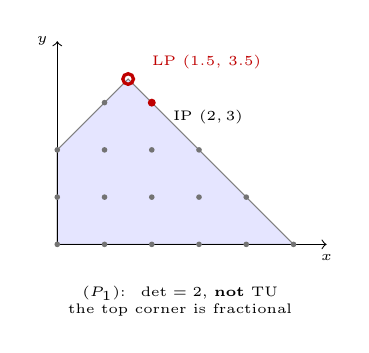
\begin{tikzpicture}[scale=0.6, font=\tiny]
  \fill[blue!10] (0,0) -- (5,0) -- (1.5,3.5) -- (0,2) -- cycle;
  \draw[thin,gray] (0,0) -- (5,0) -- (1.5,3.5) -- (0,2) -- cycle;
  \draw[->] (0,0) -- (5.7,0) node[below] {$x$}; \draw[->] (0,0) -- (0,4.3) node[left] {$y$};
  \foreach \p in {(0,0),(1,0),(2,0),(3,0),(4,0),(5,0),(0,1),(1,1),(2,1),(3,1),(4,1),(0,2),(1,2),(2,2),(3,2),(1,3),(2,3)}
    \fill[black!55] \p circle (1.7pt);
  \fill[red!75!black] (2,3) circle (2.4pt);
  \draw[red!75!black, very thick] (1.5,3.5) circle (3.2pt);
  \node[red!75!black, anchor=west] at (1.8,3.85) {LP $(1.5,\, 3.5)$};
  \node[anchor=west] at (2.25,2.7) {IP $(2,3)$};
  \node[align=center] at (2.6,-1.2) {$(P_1)$: \ $\det = 2$, \textbf{not} TU\\ the top corner is fractional};
\end{tikzpicture}
\hspace{12mm}
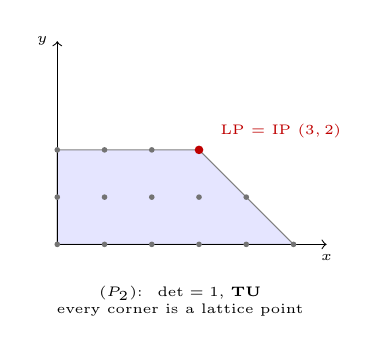
\begin{tikzpicture}[scale=0.6, font=\tiny]
  \fill[blue!10] (0,0) -- (5,0) -- (3,2) -- (0,2) -- cycle;
  \draw[thin,gray] (0,0) -- (5,0) -- (3,2) -- (0,2) -- cycle;
  \draw[->] (0,0) -- (5.7,0) node[below] {$x$}; \draw[->] (0,0) -- (0,4.3) node[left] {$y$};
  \foreach \p in {(0,0),(1,0),(2,0),(3,0),(4,0),(5,0),(0,1),(1,1),(2,1),(3,1),(4,1),(0,2),(1,2),(2,2),(3,2)}
    \fill[black!55] \p circle (1.7pt);
  \fill[red!75!black] (3,2) circle (2.6pt);
  \node[red!75!black, anchor=west] at (3.25,2.4) {LP $=$ IP $(3,2)$};
  \node[align=center] at (2.6,-1.2) {$(P_2)$: \ $\det = 1$, \textbf{TU}\\ every corner is a lattice point};
\end{tikzpicture}
\end{center}
\begin{board}
\textbf{two traps.}
\vspace{2pt}

\quad 1. a matrix of 0s and $\pm 1$s need \emph{not} be TU --- ``all my coefficients are 0/1, so my LP will come out
integral'' is a wish, not a theorem. $(P_1)$ is the counterexample
\vspace{1pt}

\quad 2. TU is a property of the matrix \emph{as a whole}, not of its rows: neither row of $(P_1)$ is guilty of anything,
the 2 appears only when you put them together. you cannot audit a model for TU one constraint at a time
\vspace{4pt}

\textbf{so how do you actually check?} \ not by determinants --- a $6 \times 9$ matrix already has thousands of square
submatrices. one checklist covers every model in this course \ (\emph{sufficient}, not necessary):
\begin{center}
\begin{tabular}{@{}l|l@{}}
 (i) & every entry is $0, \pm 1$ \\[2pt]
 (ii) & every column has at most two nonzeros \\[2pt]
 (iii) & the rows split into $M_1, M_2$ so that \textbf{in every column with two nonzeros} \\
       & the $M_1$ entries and the $M_2$ entries sum to the same thing \\
\end{tabular}
\end{center}
\vspace{2pt}

all three \ $\Rightarrow$ \ TU. \ and the whole course sits in two ways of passing (iii):
\vspace{2pt}

\quad \textbullet\ \textbf{two $+1$s in a column} (an \emph{undirected} incidence matrix): the two must land on opposite
sides, so $M_1, M_2$ is a split of the nodes with every edge crossing it --- \emph{exactly bipartiteness}
\vspace{1pt}

\quad\qquad assignment's pilot rows and aircraft rows \textbf{are} $M_1$ and $M_2$: \
\emph{the incidence matrix of a bipartite graph is TU}
\vspace{2pt}

\quad \textbullet\ \textbf{one $+1$ and one $-1$} (a \emph{directed} incidence matrix): take $M_1$ = all rows,
$M_2 = \emptyset$; \ $(+1) + (-1) = 0$ and the empty sum is 0 \ --- the networks below, and no condition on the graph at all
\vspace{4pt}

transportation has that same shape, sources on one side and sinks on the other, so it inherits the guarantee:
\begin{center}
\begin{tabular}{@{}l|l|l@{}}
 model & matrix & LP relaxation \\ \hline
 week 1's toy $(P_0)$ & a row with a 3 in it & fractional corner $(2.5, 2.5)$ \\[2pt]
 assignment & bipartite incidence, TU & integral: the LP \emph{is} the IP \\[2pt]
 transportation & bipartite incidence, TU & integral whenever $s, d$ are \\
\end{tabular}
\end{center}
\vspace{2pt}

same fact in the other vocabulary: the feasible set of assignment is the \emph{doubly stochastic} matrices, and its corners are
exactly the permutation matrices --- the honest matchings
\end{board}
\demo{demo1\_toy\_ip.py}{week 2's demo on week 1's toy, re-read with this week's eyes: the \texttt{r1}, \texttt{r2} sliders move $b$, but there is no slider for $A$ --- and $A$ is where TU lives. set \texttt{r1} $=$ \texttt{r2} $= 4$ and the LP optimum does land on $(1,1)$: failing TU means \emph{some} integer $b$ gives fractions, not every one. TU is the promise about all of them at once.}
\takeaway{first time in this course that the \emph{shape} of $A$ --- not its size, not the solver --- decided whether a problem was easy.}

% ---------------------------------------------------------------- 5
\beat{5}{Minimum cost network flow (MCNF) --- the family worth recognizing}
\demo{ip-games / min-cost-flow}{push flow through a network by hand, then let the solver do it. \ \url{https://hankpark0706.github.io/ip-games/min-cost-network-flow.html}}
\begin{board}
directed graph $G = (V, E)$: \ $V = \{1, \dots, m\}$ nodes {\footnotesize(노드)}, \ $E \subseteq \{(i,j)\}$ arcs {\footnotesize(아크)}
\vspace{3pt}

\textbf{at each node $i$:} \quad $b_i$ = net supply = outflow $-$ inflow
\begin{center}
\begin{tabular}{@{}l|l|l@{}}
 $b_i > 0$ & node $i$ supplies & \textbf{source} {\footnotesize(공급지)} \\[2pt]
 $b_i < 0$ & node $i$ demands & \textbf{destination} {\footnotesize(수요지)} \\[2pt]
 $b_i = 0$ & node $i$ only passes flow through & \textbf{transhipment}, a hub {\footnotesize(환적지)} \\
\end{tabular}
\end{center}
\vspace{2pt}

\textbf{on each arc $(i,j)$:} \ $c_{ij}$ = unit shipping cost, \ $l_{ij} \le y_{ij} \le u_{ij}$ (bounds; $0$ and $\infty$
unless the road says otherwise) \qquad \textbf{decision:} \ $y_{ij}$ = flow on arc $(i,j)$
\vspace{3pt}

\[
\begin{aligned}
  \min_{y}\quad & \textstyle\sum_{(i,j) \in E} c_{ij}\, y_{ij} \\
  \text{s.t.}\quad
    & \underbrace{\textstyle\sum_{j \,:\, (i,j) \in E} y_{ij} \;-\; \sum_{j \,:\, (j,i) \in E} y_{ji} \;=\; b_i}
        _{\text{one row per node --- \textbf{flow conservation} (흐름 보존)}}
      \quad (\forall i \in V) \\[4pt]
    & l_{ij} \le y_{ij} \le u_{ij}
\end{aligned}
\]
\vspace{1pt}

\textbf{balance is forced:} summing all rows gives 0 on the left \ $\Rightarrow$ \ $\sum_{i \in V} b_i = 0$ is required
\vspace{1pt}

\quad if the data does not balance, add a \textbf{dummy node} with zero-cost arcs to absorb the difference
\vspace{4pt}

\textbf{the matrix is the node--arc incidence matrix:} one row per node, one column per arc, $+1$ where the arc leaves,
$-1$ where it arrives
\end{board}
\begin{center}
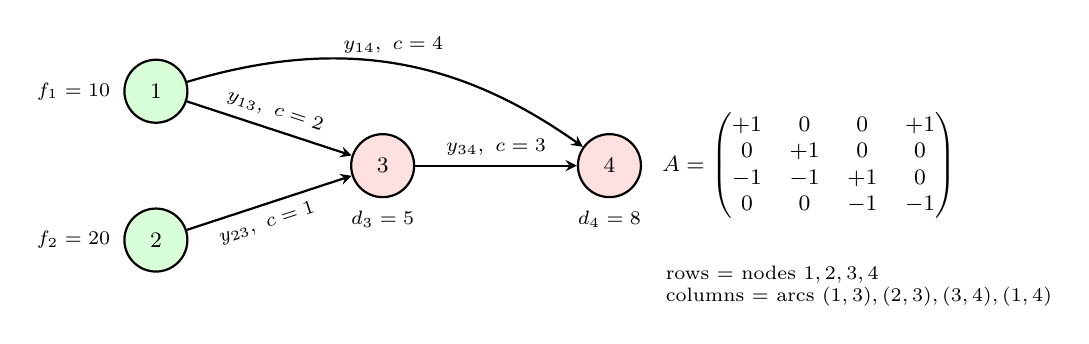
\begin{tikzpicture}[>=stealth, thick, font=\footnotesize, scale=0.9]
  \node[circle, draw, fill=green!15, minimum size=8mm] (n1) at (0, 1.5) {$1$};
  \node[circle, draw, fill=green!15, minimum size=8mm] (n2) at (0, -0.6) {$2$};
  \node[circle, draw, fill=red!12,  minimum size=8mm] (n3) at (3.2, 0.45) {$3$};
  \node[circle, draw, fill=red!12,  minimum size=8mm] (n4) at (6.4, 0.45) {$4$};
  \node[anchor=east, font=\scriptsize] at (-0.5, 1.5)  {$f_1 = 10$};
  \node[anchor=east, font=\scriptsize] at (-0.5, -0.6) {$f_2 = 20$};
  \node[anchor=north, font=\scriptsize] at (3.2, -0.05) {$d_3 = 5$};
  \node[anchor=north, font=\scriptsize] at (6.4, -0.05) {$d_4 = 8$};
  \draw[->] (n1) -- node[sloped, above, font=\scriptsize] {$y_{13}, \ c = 2$} (n3);
  \draw[->] (n2) -- node[sloped, below, pos=0.45, font=\scriptsize] {$y_{23}, \ c = 1$} (n3);
  \draw[->] (n3) -- node[above, font=\scriptsize] {$y_{34}, \ c = 3$} (n4);
  \draw[->] (n1) to[bend left=26] node[above, font=\scriptsize] {$y_{14}, \ c = 4$} (n4);
  \node[anchor=west] at (7.0, 0.45)
    {$A = \begin{pmatrix}
       +1 & 0 & 0 & +1 \\
        0 & +1 & 0 & 0 \\
       -1 & -1 & +1 & 0 \\
        0 & 0 & -1 & -1
     \end{pmatrix}$};
  \node[anchor=west, align=left, font=\scriptsize] at (7.05, -1.25)
    {rows $=$ nodes $1,2,3,4$\\ columns $=$ arcs $(1,3), (2,3), (3,4), (1,4)$};
\end{tikzpicture}
\end{center}
\begin{board}
run the checklist above on it: entries $0, \pm 1$ \checkmark, \ two nonzeros per column \checkmark, \
$M_1 = V$ and $M_2 = \emptyset$ \checkmark \ --- \emph{every} directed graph passes, with no condition on the graph
\vspace{1pt}

\quad (an \emph{undirected} edge would put two $+1$s in its column, and then only a bipartite split passes --- which is why
the \textbf{matching LP} is integral only when the graph is bipartite)
\vspace{1pt}

\quad the four rows above add to the zero row: $\det A = 0$ and $\operatorname{rank} A = 3 = |V| - 1$ --- one conservation
row is always redundant
\vspace{4pt}

\textbf{Prop.} \ integer supplies $\{b_i\}$ and integer arc bounds $\{l_{ij}\}, \{u_{ij}\}$ \ $\Rightarrow$ \ every extreme point of MCNF is
integral: the LP solves the IP, \textbf{no branching, ever}
\vspace{4pt}

\textbf{one model, four classics:}
\begin{center}
\begin{tabular}{@{}l|l@{}}
 problem & is MCNF with \\ \hline
 transportation & sources $b_i = s_i > 0$, \ destinations $b_j = -d_j$ \\[2pt]
 assignment & transportation with every $b_i = +1$, \ $b_j = -1$ (equally many of each) \\[2pt]
 shortest path & $b_s = +1$, \ $b_t = -1$, \ $b_i = 0$ otherwise \\[2pt]
 max flow & every node transhipment ($b_i = 0$); add an artificial arc $(t,s)$ and maximize $y_{ts}$ \\
\end{tabular}
\end{center}
so assignment and transportation were the same model twice --- and both were networks
\vspace{4pt}

\textbf{the picture above is not yet an MCNF instance.} nodes 3 and 4 are destinations ($b_3 = -5$, $b_4 = -8$), so nodes 1
and 2 must supply 13 between them --- \emph{which one, and how much, is not data.} that is the LAP, two sections down
\end{board}
\key{if you can \emph{recognize} an IP as a network, it is solved: one row per node, one column per arc, $\pm 1$ entries --- TU by construction.}

% ---------------------------------------------------------------- 6
\beat{6}{Facility location --- paying to open}
\begin{board}
transportation assumed the depots were already there, holding $s_i$ tons apiece. the planning question that actually costs
money comes first: \emph{which depots should exist at all?} {\footnotesize(시설 입지 문제)}
\vspace{3pt}

one new decision, one new cost: \quad
$x_i = \begin{cases} 1 & \text{depot $i$ opens} \\ 0 & \text{otherwise} \end{cases}$
\qquad $f_i$ = fixed cost of opening depot $i$
\[
\begin{aligned}
  \min_{x,\,y}\quad & \textstyle\sum_{i} f_i x_i \;+\; \sum_{i} \sum_{j} c_{ij} y_{ij}
    && \text{fixed cost $+$ shipping cost} \\
  \text{s.t.}\quad
    & \textstyle\sum_{i} y_{ij} = d_j && \text{(demand)} \\
    & y_{ij} \le M x_i && \textbf{(linking --- week 2)} \\
    & y_{ij} \ge 0, \quad x_i \in \{0,1\}
\end{aligned}
\]
read the linking row: \ $x_i = 0 \Rightarrow y_{ij} = 0$ (a closed depot ships nothing); \ $x_i = 1$ releases it entirely
--- which is what \emph{un}capacitated means
\vspace{2pt}

\quad \emph{how big is $M$?} \ week 2's craft applies on the spot: this row governs one $(i,j)$ pair, and no plan ever
ships more than $d_j$ to sink $j$, so $M = d_j$ is valid and smallest. \ ($M = \sum_j d_j$ is also valid --- and on a
two-depot instance costs 5 points of LP bound for nothing.)
\vspace{4pt}

\textbf{1. fix $x$ and transportation falls out.} \ if somebody tells you which depots are open, $\sum_i f_i x_i$ is a
constant and the linking rows become plain bounds; what is left is transportation. \ \emph{all the hardness is in the binaries}
\vspace{3pt}

\textbf{2. the big-$M$ row costs you the guarantee.} \ transportation's matrix was a bipartite incidence matrix; the row
$y_{ij} \le M x_i$ belongs to no incidence matrix at all. the MCNF proposition no longer applies
\vspace{1pt}

\quad by trap 1 that is not yet a proof that the LP \emph{will} lie --- so the next section goes and checks
\end{board}
\key{every guarantee in this note is a property of $A$ --- so every guarantee is one modeling decision away from being lost.}

% ---------------------------------------------------------------- 7
\beat{7}{The LAP --- when $b$ is a decision}
\begin{board}
MCNF takes the supplies $b_i$ as data. the \textbf{location--allocation problem} {\footnotesize(입지-배분 문제)} does not:
\emph{we choose them}
\vspace{3pt}

\quad $r_i \ge 0$ = reserve pre-positioned at node $i$ (holding cost $h_i$/ton), \quad $q_i \ge 0$ = unmet demand
(penalty $u_i$), \quad $s_i \ge 0$ = surplus (penalty $o_i$)
\[
  b_i \;=\; \underbrace{r_i}_{\text{decision}} \;-\; d_i \;+\; q_i \;-\; s_i
  \qquad\Longrightarrow\qquad
  \underbrace{\textstyle\sum_{j} y_{ji} - \sum_{j} y_{ij}}_{\text{inflow} \;-\; \text{outflow}}
  \;+\; r_i + q_i - s_i \;=\; d_i \quad (\forall i \in V)
\]
that is the whole difference between a network flow problem and the LAP: \ \textbf{$b$ is not given to us}
\vspace{3pt}

\[
\begin{aligned}
  \min_{x,\,r,\,y,\,q,\,s}\quad
    & \textstyle\sum_{i} f_i x_i + \sum_{i} h_i r_i + \sum_{(i,j) \in E} c_{ij} y_{ij}
      + \sum_{i} u_i q_i + \sum_{i} o_i s_i \\
  \text{s.t.}\quad
    & \textstyle\sum_{j} y_{ji} - \sum_{j} y_{ij} + r_i + q_i - s_i = d_i && (\forall i) && \text{[conservation --- MCNF]} \\
    & \textstyle\sum_{i \in S} r_i \le B && && \text{[budget --- one knapsack row]} \\
    & r_i \le B\, x_i && (\forall i \in S) && \text{[linking --- week 2]} \\
    & \textstyle\sum_{i \in S} x_i \le p && && \text{[at most $p$ depots --- week 2]} \\
    & y, r, s \ge 0, \quad 0 \le q_i \le d_i, \quad x_i \in \{0,1\}
\end{aligned}
\]
five costs: \ open ($f_i$), \ hold ($h_i$), \ ship ($c_{ij}$), \ fail ($u_i$), \ waste ($o_i$)
\vspace{1pt}

\quad $S \subseteq V$ = the \textbf{candidate sites}; elsewhere $x_i = r_i = 0$ --- you do not stock reserve inside the
disaster area
\vspace{1pt}

\quad \emph{every constraint is old}, and $M = B$ passes in the linking row because the budget row already caps every
$r_i$ at $B$ --- valid, though week 2 would ask whether it is the \emph{smallest} valid $M$
\end{board}
\begin{board}
the network above, priced --- $S = \{1,2\}$, \ $B = 15$, \ $p = 1$, \ $h_i = 1$, \ $u_i = 100$, \ $o_i = 1$:
\[
\begin{aligned}
  \min\quad & 10 x_1 + 20 x_2 + r_1 + r_2 + 2 y_{13} + y_{23} + 3 y_{34} + 4 y_{14}
    + 100 (q_3 + q_4) + \textstyle\sum_i s_i \\
  \text{s.t.}\quad
    & -y_{13} - y_{14} + r_1 + q_1 - s_1 = 0 && \text{[node 1]} \\
    & -y_{23} + r_2 + q_2 - s_2 = 0 && \text{[node 2]} \\
    & y_{13} + y_{23} - y_{34} + q_3 - s_3 = 5 && \text{[node 3]} \\
    & y_{34} + y_{14} + q_4 - s_4 = 8 && \text{[node 4]} \\
    & r_1 + r_2 \le 15, \qquad r_1 \le 15 x_1, \qquad r_2 \le 15 x_2, \qquad x_1 + x_2 \le 1 \\
    & y, r, s \ge 0, \quad 0 \le q_3 \le 5, \quad 0 \le q_4 \le 8, \quad x_1, x_2 \in \{0,1\}
\end{aligned}
\]
sixteen variables, two of them binary --- and $q_1 = q_2 = 0$ is forced by $q_i \le d_i$, so fourteen really move.
\ every number came off the picture. \ at $p = 1$ there are two plans:
\begin{center}
\begin{tabular}{@{}l|c|c|l|c@{}}
 plan & open & hold & ship & total \\ \hline
 $x_2 = 1$: \ $r_2 = 13$, \ $y_{23} = 13$, \ $y_{34} = 8$ & $20$ & $13$ & $1 \cdot 13 + 3 \cdot 8 = 37$ & $70$ \\[2pt]
 $x_1 = 1$: \ $r_1 = 13$, \ $y_{13} = 5$, \ $y_{14} = 8$ & $10$ & $13$ & $2 \cdot 5 + 4 \cdot 8 = 42$ & $\mathbf{65}$ \\
\end{tabular}
\end{center}
site 2 ships cheaper and still loses: it would save 5 on the road and pay 10 more at the door
\vspace{1pt}

\quad the gap is entirely city 3 (5 tons at 1/ton against 2/ton); on city 4 the two sites are exactly tied ---
4/ton direct from site 1 against $1 + 3$ through the hub from site 2
\vspace{1pt}

\quad raise $f_1$ to 15 and the two tie at 70; \ past that, or with the bypass arc $(1,4)$ flooded (site 1 then pays
$2 \cdot 13 + 3 \cdot 8 = 50$ to ship, total 73), site 2 wins
\vspace{2pt}

\quad \textbf{that trade --- a cost paid once against a cost paid per ton --- is the LAP}
\vspace{4pt}

\textbf{and the LP? it lies, exactly as the big-$M$ row warned:}
\[
  z_{\mathrm{LP}} = 62 \quad < \quad z_{\mathrm{IP}} = 65,
  \qquad\text{at}\quad x_1 = \tfrac{8}{15}, \ \ x_2 = \tfrac13, \ \ r_1 = 8, \ \ r_2 = 5
\]
\quad it buys eight-fifteenths of depot 1 and a third of depot 2, pays $10 \cdot \tfrac{8}{15} + 20 \cdot \tfrac13 = 12$ to
open instead of 10, then serves city 3 from site 2 at 1/ton \emph{and} city 4 from site 1 at 4/ton --- a shipping bill of 37
that no single depot can achieve. \ $12 + 13 + 37 = 62$
\vspace{1pt}

\quad half-open depots are not a plan, and the $12$ is not a price anyone can pay. \ \emph{that} is what losing TU costs
\end{board}
\demo{lap\_app.py}{this model on a map --- and a head start on week 9, since the dashboard fits the plan to \emph{several} sampled disasters: drag \texttt{training data} down to 1 and it collapses to today's single-scenario model. \texttt{max facilities} is $p$, and the prices are $B$ (\texttt{budget B}), $f_i$ (\texttt{facility cost c}), $h_i$ (\texttt{reserve cost f}) --- the app's letters do not line up with ours. \emph{Solve} picks the plan, \emph{Simulate disaster} routes it against one demand draw; leave \emph{SAA vs mean} alone, that button is week 9.}
\takeaway{LAP $=$ MCNF $+$ two decisions MCNF cannot make: \emph{which} nodes supply ($x_i$) and \emph{how much} ($r_i$). fix those two and a network flow problem is all that is left --- TU, easy. all the hardness is in $(x, r)$.}

% ---------------------------------------------------------------- 8
\beat{8}{The assumption we just made}
\begin{board}
look at where $d_i$ sits in the model: on the right-hand side, \emph{known}. \ and look at when we choose $x_i$ and $r_i$:
in the same model, at the same moment, as $y_{ij}$ and $q_i$
\vspace{2pt}

\quad so the model assumes you know each city's demand \emph{when you decide where to build}. nobody knows where the
earthquake will be
\vspace{4pt}

the real sequence has a gap:
\begin{center}
\begin{tabular}{@{}l|c|l@{}}
 \textbf{stage 1: now} & \emph{$\longrightarrow$ \ the disaster \ $\longrightarrow$} & \textbf{stage 2: then} \\ \hline
 open depots, place stock & demand $d$ reveals itself & route what you have \\[2pt]
 $x_i$, \ $r_i$ & & $y_{ij}$, \ $q_i$, \ $s_i$ \\[2pt]
 committed, binary, expensive & & reactive, a flow problem, easy \\
\end{tabular}
\end{center}
\vspace{2pt}

the split is the one the model above already found \emph{in the variables} --- the model does not need rebuilding, it needs re-reading
\vspace{3pt}

what ``optimal'' means across that gap is the open question: plan for the worst case and you build for an earthquake that
never comes; plan for the average and note that the average disaster never happens
\vspace{2pt}

\quad no formulation today --- that is week 9, and it needs the weeks in between first
\end{board}
\key{\emph{ML predicts; optimization decides} --- a forecast of $d$ is an input, not an answer.}

% ---------------------------------------------------------------- next
\enlargethispage{3\baselineskip}
\par\medskip
{\color{ruleink}\rule{\textwidth}{1.2pt}}\par\nobreak\vspace{3pt}
{\color{keyink}\small\textbf{next lecture}\quad is $r_i \le B x_i$ the \emph{best} way to write that row? other formulations
describe the same plans and return the same answer --- and one solves in seconds where another runs all night.
\ \textbf{Homework 2 is out} (due 10/6).}

\end{document}
